Esta fase sirve no solo para obtener los datos sino también para conocer las
características de los datos así como su preparación previa antes de ser usados
(en el caso de datos personales), sino también para generar todos los
desarrollos requeridos en otras áreas tanto de software u organizacionales para
la adquisición y posterior procesamiento de estos datos. Esto incluye la
creación de Bases de Datos Relacionales o No Relacionales, conexión a servidores
remotos; pero no se limita a ello, sino también tener métodos efectivos de
captura de datos, en casos donde estos se generen de forma manual o se
encuentren en papel. En el caso de las imágenes, también se tiene que idear la
forma de su captura y posterior utilización. Saber si se va a trabajar con
imágenes, series de tiempo, archivos de excel, valores categóricos, continuos o
discretos es uno de los factores más importantes para la elección de un
algoritmo que soluciones el problema. 

\subsection{Determinar datos necesarios}

Como regla general, se prefiere tener tantos datos posibles\footnote{Más datos
es mejor rendimiento.}, es decir, filas en un archivo tabular ya que datos
variados y una base de datos grande permiten un mejor entrenamiento de cualquier
algoritmo. Pero también se requiere juntar la mayor cantidad de característica,
columnas, para determinar cuales de estas inciden en la etiqueta de salida; en
fases subsecuentes se reducirá este conjunto de atributos mediante técnicas para
escoger los más importantes y significativos.

Los datos necesarios para esta tesis deben ser: imágenes tomadas con un
microscopio dentro de un \hyperlink{abbr}{PAP}, correctamente clasificadas y
validadas en protocolos de análisis citológico.

\subsection{Capturar u obtener datos}

La captura de datos es un proceso complejo, requiere un diseño de experimentos
completo y manejo de condiciones estadísticas adecuadas para asegurar un
conjunto de datos representativo del problema a resolver. En los problemas de
clasificación, es preferible que el número de datos por clase sea balanceado;
esto no siempre es posible, por ejemplo, en aplicaciones médicas es habitual
tener más datos de ausencia de enfermedad que de enfermedad.

Hay que tener consideración especial en la variedad de los datos. Por ejemplo,
si se quieren clasificar perros y gatos, habría que conseguir imágenes de todas
las razas de ambos animales, de todos los tamaños y en condiciones distintas de
captura de la imagen con el objetivo de maximizar la capacidad de clasificación
del mismo. Una analogía de esto es aprender a resolver ejercicios matemáticos,
si nos limitamos a resolver solamente los de un libro en particular, careceremos
de un aprendizaje real de las matemáticas, nos volveremos expertos en un libro y
seremos incapaces de generalizar el conocimiento.

La \hyperlink{abbr}{BD} DTU/Herlev\footnote{\url{http://mde-lab.aegean.gr/index.php/downloads}}, del doctor Jan Jantzen
ha sido compilada durante más de 10 años con imágenes normales y anormales de
\hyperlink{abbr}{PAP}s provenientes del Hospital Universitario de Herlev en
Dinamarca, gracias al Dr. M.D. Beth Bjerregaard. El análisis de esta
\hyperlink{abbr}{BD} fue realizado a través de muchas tesis de maestría en el
laboratorio de automatización de esta universidad y con el doctor G. Dounias en
la Universidad del Mar Egeo en Grecia~\cite{MBE-LAB}~\cite{Jantzen2005}. 

Ellos amablemente proveyeron los datos para esta tesis. Que consiste en un
conjunto de imágenes clasificadas y validadas por expertos así como la
documentación requerida para entenderla. Incluyendo las tesis de maestría y
ligas a otros experimentos e investigaciones hechas con la \hyperlink{abbr}{BD}.
Lo cual le dio un empuje muy grande a la realización de esta tesis.

Dada la gran cantidad de laminillas generadas, se creó una \hyperlink{abbr}{BD}
basada en imágenes individuales. Expertos cito-tecnólogos utilizando
microscopios a una resolución de \(0.201  \frac{\mu}{pixel}\) para capturar imágenes
digitales. Cada imagen es después clasificada en siete clases en un proceso de
validación que consiste en repetir el análisis con dos cito-tecnólogos
distintos. Si la validación resultaba negativa la célula era descartada~\cite{Norup2005}~\cite{Martin2003}. 

El archivo comprimido contiene:

\begin{itemize}
    \item El artículo Pap-smear Benchmark Data For Pattern Classification donde se explica
    la necesidad y la creación de una base de datos de \hyperlink{abbr}{PAP} para ser usada como benchmark
    para probar algoritmos de clasificación; con el objetivo de permitir a estudiantes e investigadores
    el acceso a una \hyperlink{abbr}{BD} validada~\cite{Jantzen2005}.
    \item La tesis Pap-Smear Classification, donde se propone un método basado en extracción
    de características y el algoritmo Fuzzy C-means, utilizando validación cruzada~\cite{Martin2003}.
    \item La tesis Classification of pap-smear data by transductive neuro-fuzzy
    methods, que utiliza algoritmos neuro difusos y KNN, en la misma \hyperlink{abbr}{BD}~\cite{Norup2005}.
    \item La carpeta con las imágenes, dividida en subcarpetas.
    \item Un archivo de Excel que contiene el nombre del archivo de imagen, las características
    extraídas y la clase a la que pertenece.
\end{itemize}

\subsection{Crear repositorios}

Un repositorio es un lugar seguro donde almacenar los datos y provee una
estructura para mantener un correcto control tanto de los datos como del código
usado para explorar, procesar, entrenar y evaluar.

Los repositorios de datos estarán divididos en dos: 

\begin{itemize}
    \item{Local:} Almacenados en un Disco de Estado Sólido local con conexión de
    3000 MB/s de lectura.
    \item{Nube:} Divididos entre un sistema de almacenamiento en la nube y un repositorio
    de datos para control de versiones\footnote{\url{https://github.com/marcojulioarg}}.
\end{itemize}

El repositorio local es donde se almacenará la \hyperlink{abbr}{BD} aumentada,
que contendrá miles de imágenes y su peso rondará los gigabytes.

El repositorio remoto y sistema de almacenamiento guardará el código, que se
compone de \emph{Jupyter Notebooks} legibles y explicados para replicar el
experimento. Este repositorio está designado de libre acceso y todos pueden
descargarlo y analizar el código que generó los resultados de esta tesis\footnote{\url{https://github.com/marcojulioarg/ConvoPap}}.

\subsection{Crear entorno de trabajo}

El entorno de trabajo se refiere a la configuración del equipo de cómputo, a la
instalación de software y módulos necesarios para hacer \hyperlink{abbr}{ML}.
Este entorno no solo sirve para hacer el trabajo, sino también para facilitar su
distribución y orden integrando documentos digitales con código y comentarios en
formato legible; capaz de integrar multimedia y ser compartidos fácilmente.

Se pensó en la manera más sencilla de crear el entorno de trabajo, es por ello
que se prefieren métodos de instalación gráficos en comparación a los métodos
basados en consola para permitir el entendimiento por personas no versadas en el
área computacional.

\subsubsection{\emph{Jupyter Notebooks}}

Proyecto Jupyter es de código abierto sin ánimos de lucro, creado en 2011 para
trabajar interactivamente en las comunidades de científicas y computacionales.
Sus creadores observaron que los científicos de datos tenían problemas para
compartir descripciones detalladas y entendibles de su código a sus colegas. 

Son documentos digitales basados en la web que sirven para escribir código,
documentarlo, correrlo, visualizar datos y exportarlos sin salir del mismo
entorno. Es una herramienta poderosa para aplicar cualquier metodología tanto de
\hyperlink{abbr}{ML} como de ciencia de datos.

En la \autoref{fig:jupyter} podemos apreciar la interface. Podemos ver que se
pueden insertar hipervínculos (así como video o imágenes), puede renderizar
código \LaTeX{} para generar ecuaciones ricas y precisas. La ejecución del código
está dividida en celdas, donde cada celda se ejecuta de manera individual y
muestra su resultado inmediatamente, estos resultados pueden ser tanto
numéricos, tablas o figuras y gráficas como se observa.

Se crearán \emph{Jupyter Notebooks} para cada una de las siguientes fases de la
metodología, con el objetivo de que estas se puedan seguir paso por paso para un
mejor entendimiento.

\begin{figure}[H]
    \centering
    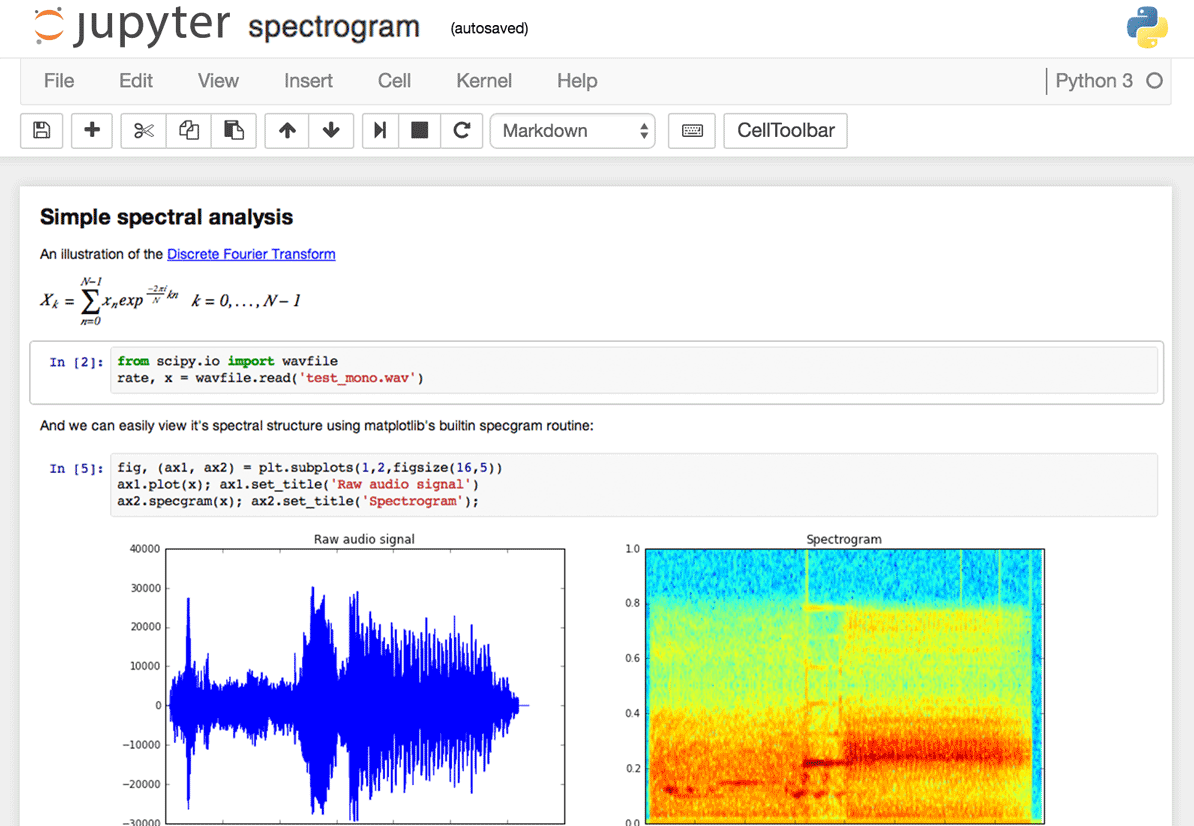
\includegraphics[width=0.8\textwidth]{capitulo_sdac/jupyter}
    \caption{Interface de un \emph{Jupyter Notebook}}\label{fig:jupyter}
\end{figure}
    
\subsubsection{Configuración}

Como intérprete de Python se utilizará la distribución de \emph{Anaconda}, de
código abierto, especialmente compilada para su uso en cómputo científico. Tiene
la mayoría de módulos necesarios para iniciar un análisis de datos o un
experimento de \hyperlink{abbr}{ML}. Para instalarlo, es necesario ir al sitio
web de \href{https://www.anaconda.com/distribution/}{Anaconda} e instalar la
versión de 64
bits\footnote{\url{https://www.anaconda.com/distribution}}.

Se procede a crear un entorno virtual de trabajo, este crea un intérprete
independiente para un mejor control del proyecto. Para interactuar con Anaconda,
se utiliza la interface gráfica Anaconda Navigator, donde podremos gestionar
varios intérpretes virtuales (\autoref{fig:anaconda}).

\begin{figure}[H]
    \centering
    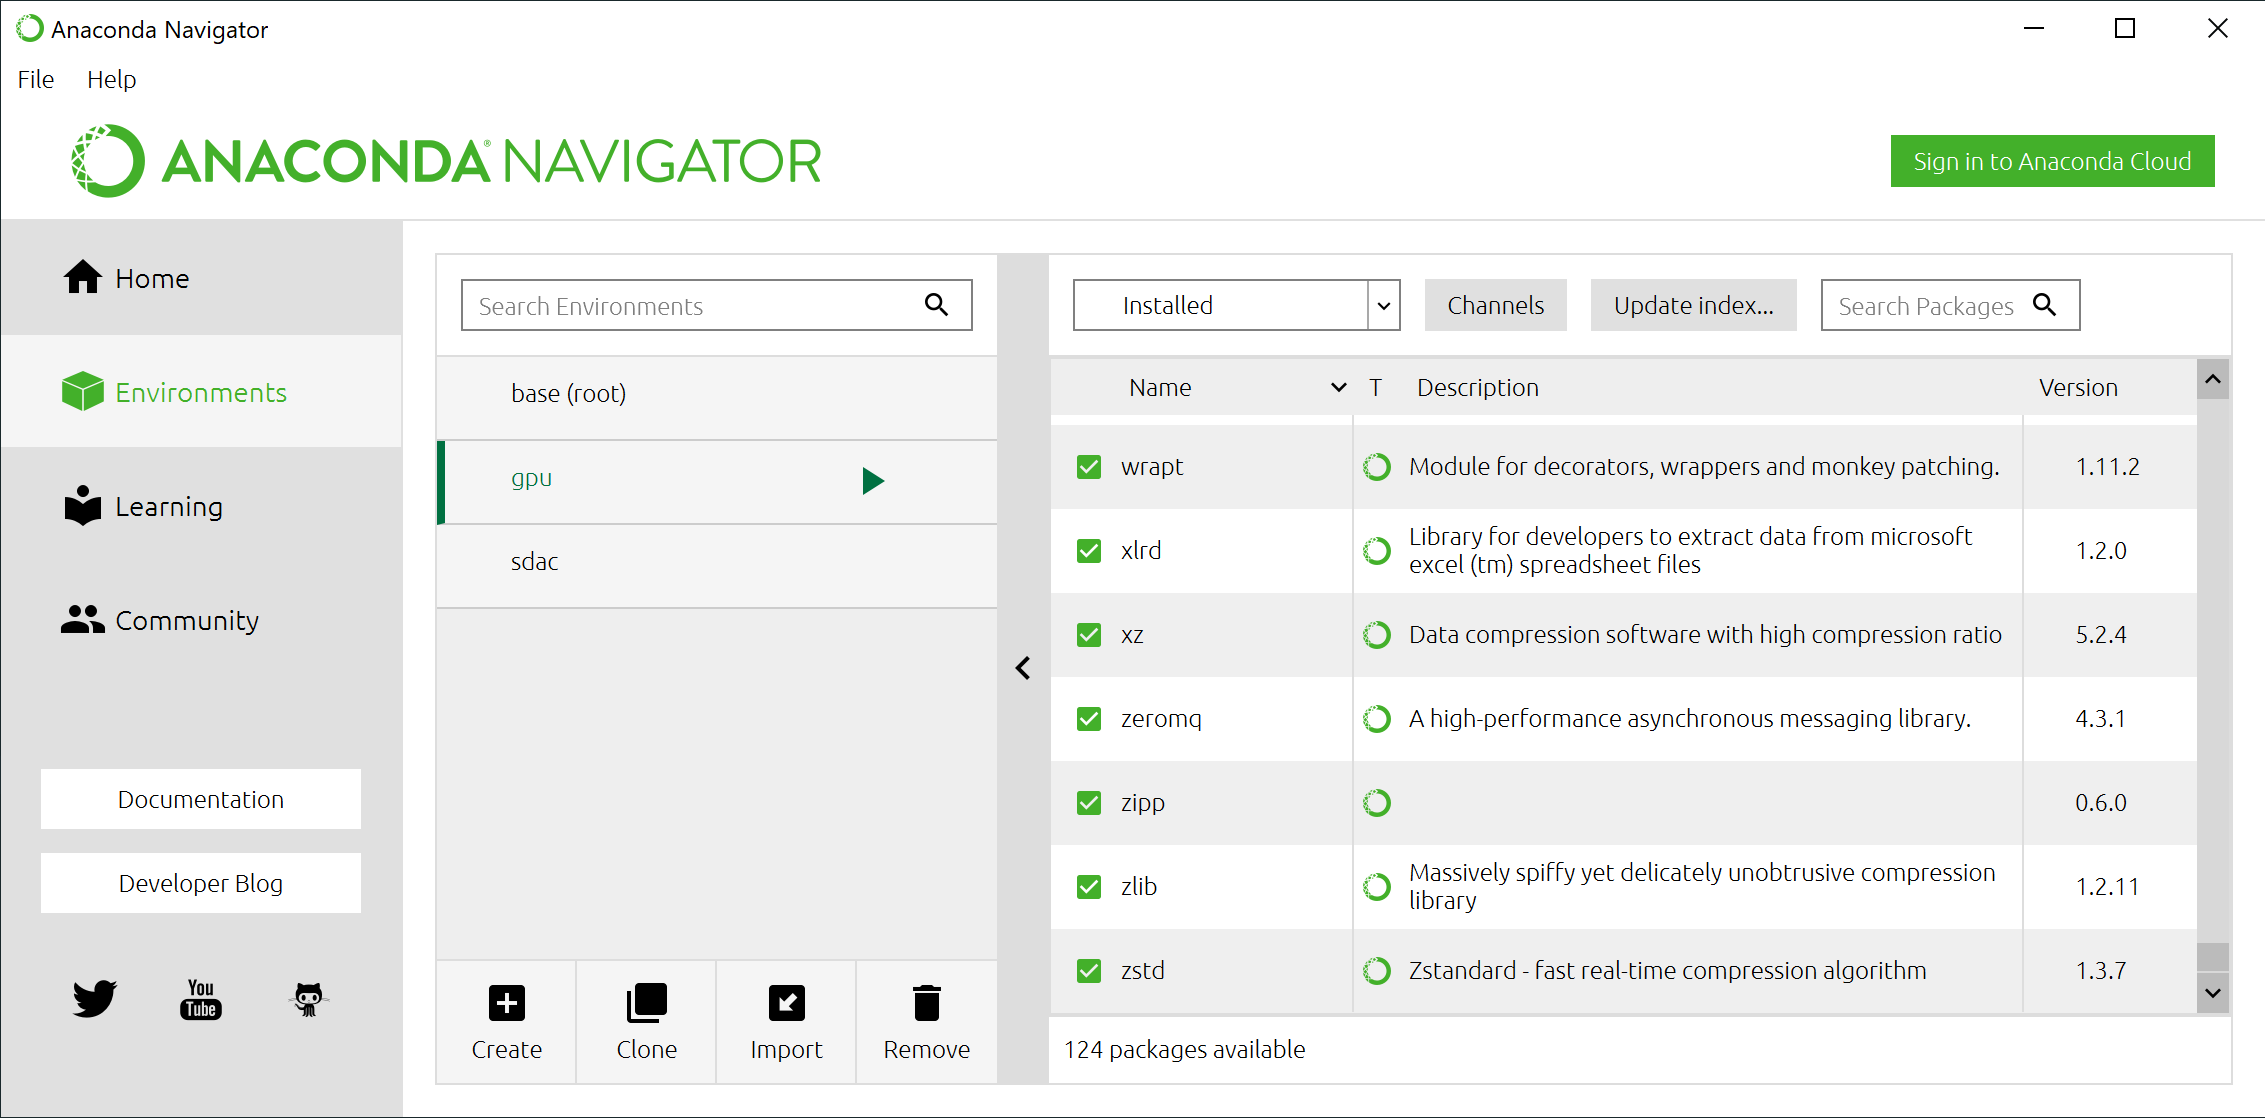
\includegraphics[width=0.8\textwidth]{capitulo_sdac/anaconda}
    \caption{Anaconda Navigator}\label{fig:anaconda}
\end{figure}

Para poder instalar el software de \hyperlink{abbr}{DL}, es necesario haber
instalado previamente los \emph{Drivers} para el \hyperlink{abbr}{GPU} en caso
de que se tenga uno. Configurar este dispositivo para cambiar su propósito de
procesamiento gráfico a procesamiento general es una maraña de instalaciones y
softwares auxiliares, afortunadamente, Anaconda tiene una forma sencilla de
instalar y configurar \textbf{Tensorflow} con todas sus
dependencias\footnote{\mintinline{latex}{conda install -c anaconda
tensorflow-gpu}}.

A continuación enumeraremos algunos módulos de python relevantes para la creación
del entorno de desarrollo:

\begin{enumerate}
    \item{\textbf{Jupyter: }} Permite el uso de documentos digitales.
    \item{\textbf{OpenCV: }} Módulo para \hyperlink{abbr}{PDI} y \hyperlink{abbr}{VC}.
    \item{\textbf{Pandas: }} Sirve para manipular datos tabulares.
    \item{\textbf{Numpy: }} Módulo para cómputo matemático.
    \item{\textbf{Sklearn: }} Módulo de \hyperlink{abbr}{ML} y Ciencia de Datos.
    \item{\textbf{Matplotlib: }} Para hacer gráficas y figuras.
    \item{\textbf{Tensorflow: }} Para entrenar el modelo.
\end{enumerate}

\subsection{Datos}

Terminando este proceso obtendremos una carpeta de datos, con subcarpetas para
cada clase con un peso de 100MB que posteriormente exploraremos para determinar
sus características para luego transformarse en conocimiento.

Así mismo, concluimos la instalación y configuración del entorno de trabajo
computacional. El cual nos servirá para continuar con las siguientes etapas y
generará código capaz de ser revisado, probado y replicado. 